\documentclass[11pt, a4paper]{article}
\usepackage{graphicx} % Required for inserting images
\usepackage{array}
\usepackage{booktabs}
\usepackage[
        backend=biber,
        style=apa,
        sorting=nyt,
    ]{biblatex}
\addbibresource{references.bib}
\usepackage{float}
\usepackage[colorlinks=true, urlcolor=blue, linkcolor=black, citecolor=black]{hyperref}
\usepackage{minted}
\usepackage[margin=1in]{geometry}
\begin{document}
\begin{figure}[h]

\includegraphics[width=7cm]{Figures/logo_kul.png}
\end{figure}
\vspace*{5cm}

\begin{center}
\hrule 
\vspace{0.5cm}
\noindent
\huge{\textbf{Comparative Genomics: Frizzled Receptors}} \\ 
\vspace{1cm}
\hrule 
\vfill
\end{center}

\begin{flushright}
\large{William Mwine} \\
\large{r0993335} \\
\normalsize{Master of Bioinformatics} \\
\normalsize{Academic year 2024-2025}
\end{flushright}

\vspace{1cm}


\section{Introduction}
\label{intro}
Frizzled proteins are transmembrane proteins that play a key role in the Wnt signaling pathway as well as other signaling pathways. They bind to Wnt proteins and pass the signal to dishevelled proteins during the signaling process. At their extracellular amino terminus, frizzled proteins have a cysteine-rich domain that binds Wnt ligands, while the intracellular carboxyl terminus contains a KTXXXW motif essential for Wnt signaling. \cite{Huang2004-zi}. These features are highly conserved across species highlighting their importance. In this analysis, I will focus on the Frizzled 7(FZD7) protein, investigating its conservation across species. This  study aims to provide insights into its evolutionary history and the preservation or diversification of its function over time.
\section{Methods}
\label{BigMethods}
\subsection{Sequences}
\label{seq-meth}
The sequences used for the downstream analyses were acquired by searching for homologs of the human FZDZ protein. These homologous sequences were obtained using the NCBI BLASTP tool with default settings, except for the \texttt{max\_target\_seqs} parameter, which was set to 250 to retrieve up to 250 sequences. The results were then filtered to remove synthetic constructs, low-quality sequences, and predicted sequences. From the remaining sequences, 100 were randomly sampled and used for downstream analyses.
\subsection{Multiple sequence alignment}
\label{msa-meth}
The multiple sequence alignment (MSA) was constructed using \texttt{ClustalW2} with the slow and accurate parameter.
\subsection{Phylogenetic Tree construction}
\label{tree-meth}
The phylogenetic tree of the sequences from \autoref{seq-meth} was constructed using IQ-TREE multicore version 2.3.6. IQ-TREE determined the best model for the MSA to be \texttt{Q.mammal+I+G4} based on the Bayesian Information Criterion (BIC). This model uses the \texttt{Q.mammal} amino acid exchange rate matrix \cite{Minh2021-yc} along with an invariable site plus discrete Gamma model to account for rate heterogeneity across sites. \\
To annotate this tree with evolutionary events like duplication and speciation, a species tree of the species of the FZD7 protein sequences from \autoref{seq-meth} was contructed. As recommended by \cite{Tobe2010-bi}, the mitochondrial \textit{cytochrome b} (\textit{cyt b}) gene was used to construct the species tree due to its sufficient intraspecific and interspecific variation, which enables effective species differentiation. Whole mitochondrial genome sequences were obtained from \href{https://www.ncbi.nlm.nih.gov/}{NCBI}. The \textit{cyt b} gene was then extracted from these sequences and used to construct an MSA using clustaw. Similar to \autoref{tree-meth}, IQ-TREE was used to select the best model for our MSA based on the Bayesian Information Criterion (BIC). The \texttt{GTR+F+I+R5} model, with 1000 bootstraps, was selected. This model uses the General Time Reversible (GTR) substitution model with unequal rates and unequal base frequencies, along with empirical base frequencies, and accounts for invariable sites plus a FreeRate model. This model was then used to construct the species tree. \\
The FZD7 protein tree was then annotated using Notung-2.9 by \cite{Stolzer_Lai_Vernot_Darby_Xu_Goldman_Sathaye_Durand} and is based on algorithms \cite{Stolzer2012},\cite{Darby2016},\cite{Durand2006},\cite{Lai2017},\cite{Vernot2008}
\subsection{Conserved regions}
Jalview \cite{Jalview2024} was used to visualize the FZD7 sequence alignment and to calculate Thompson conservation scores \cite{Thompson1999} for all columns.
\section{Results}
\begin{figure}[H]
    \centering
    
\includegraphics[width=\linewidth]{Figures/FZDZ-seq.aln.contree.png} 
    \caption{Phylogenetic tree of Frizzled 7 protein sequences. Nodes labeled with "D" represent duplication events, while unlabelled nodes indicate speciation events. The shape of the nodes reflects bootstrap values: nodes with clear shapes have high bootstrap values (greater than 90), while unclear or absent node shapes correspond to bootstrap values below 50.This tree demonstrates the evolutionary relationships and gene duplication events in FZD7 receptors}
    \label{figure1-FZD7-tree}
\end{figure}
The phylogenetic tree of the FZD7 sequences shown in Figure 1 has terminal leaves with high bootstrap values, although a few internal nodes exhibit low values, with the lowest being 11. Out of all the nodes, 40 are annotated as duplication events, while the remaining nodes represent speciation events. Figure 2 depicts the species tree used for reconciliation of the FZD7 phylogenetic tree, including rooting and annotation of duplication and speciation events. This species tree clearly displays distinct clades separating the species.
\begin{figure}[h]
    \centering
    
\includegraphics[width=0.8\linewidth]{Figures/Cytb_seq-2.aln.contree.png} 
    \caption{Species Tree used for reconciliation of FZD7 tree shown in \autoref{figure1-FZD7-tree}. The tree was constructed using mitochondrial \textit{Cytochrome b} genes. Distinct clades represent species-specific groups, and node values indicate bootstrap support, representing the confidence level of each node.}
    \label{fig:example-image}
\end{figure}

\noindent Table 1 shows conservation analysis of the FZD7 MSA. Highlighting conserved regions as well as their respective functions.
\begin{table}[H]
\begin{tabular}{|l|l|l|l|l|l|}
\hline
\textbf{Region} & \textbf{Position} & \textbf{\begin{tabular}[c]{@{}l@{}}Consesus\\ Logo\end{tabular}} & \textbf{\begin{tabular}[c]{@{}l@{}}Conservation\\  score\end{tabular}} & \textbf{GO:Terms} & \textbf{Function} \\ \hline
region1 & 47-164 & \autoref{fig:CRD-logo} & 0.98 & \begin{tabular}[c]{@{}l@{}}GO:0017147, \\ GO:0042813\end{tabular} & \begin{tabular}[c]{@{}l@{}}Wnt protein binding, \\ Wnt receptor activity\end{tabular} \\ \hline
region2 & 206-549 & \autoref{fig:hydroDomains-logo} & 0.99 & \begin{tabular}[c]{@{}l@{}}GO:0004888,\\ GO:0042813\end{tabular} & \begin{tabular}[c]{@{}l@{}}transmembrane \\ signaling \\ receptor activity,\\ Wnt receptor activity\end{tabular} \\ \hline
region3 & 552-557 & \autoref{fig:KTXXXW motif-logo} & 1.0 &  & \begin{tabular}[c]{@{}l@{}}activation of the \\ Wnt-$\beta$-catenin\\ pathway \cite{Huang2004-zi}\end{tabular} \\ \hline
\end{tabular}
\caption{Conserved Regions Analysis. This table lists key conserved regions in the FZD7 protein, their positions, average Thompson conservation scores, and associated functional roles. The consensus logos (Figures 3-5) illustrate sequence conservation in these regions.}
\label{Table-1-conservation}
\end{table}

\section{Discussion}
From the analysis of FZD7 receptors, an evolutionary history characterized by both duplication and speciation events can be seen. Duplication events have led to the emergence of paralogs, which subsequently underwent processes such as neofunctionalization, specialization, subfunctionalization, or other evolutionary fates. As depicted in \autoref{figure1-FZD7-tree}, the FZD7 protein in Homo sapiens is a paralog to FZD7 proteins from primate species like \textit{Gorilla gorilla gorilla} (western lowland gorilla) and \textit{Pongo abelii} (Sumatran orangutan), as well as species like \textit{Canis lupus familiaris} (domesticated dog). Isoforms are however also annotated as paralogs in the phylogenetic tree forexample FZD7 isoformX1 and FZD7 isoformX2 from the Eurasian otter (\textit{Lutra lutra}). However, this classification is inconsistent with the evolutionary definition of paralogs. Isoforms are distinct proteins produced from the same gene through alternative splicing of pre-mRNA while paralogs arise from duplicated genes. Orthologous relationships are observed with FZD7 proteins from species such as \textit{Sapajus apella} and \textit{Trachypithecus francoisi}.

\noindent The conservation of FZD7 function across diverse species highlights the critical role of frizzled receptors. As mentioned in \autoref{intro}, frizzled receptors are integral to Wnt signaling, which regulates the expression of genes involved in cell proliferation and differentiation \cite{Liu2022-kj}.

\noindent The conserved regions of FZD7 are shown in \autoref{Table-1-conservation}, along with their respective functions. Region 1 represents the cysteine-rich domain, which is highly conserved in frizzled receptors across species. This domain is responsible for the binding of Wnt ligands \cite{Huang2004-zi}. Region 2 refers to the seven linked transmembrane hydrophobic domains, and just after it is Region 3, which denotes the KTXXXW motif. Region 3 plays a role in the activation of the Wnt-$\beta$-catenin pathway \cite{Huang2004-zi}.

\noindent In conclusion, this analysis reveals a rich evolutionary history of FZD7 receptors marked with duplication and speciation events. Despite these evolutionary events, FZD7 has preserved its function across species with key conserved regions such as the cystein rich domain and KTXXXW motif which play crucial roles in Wnt signaling.
\printbibliography
\appendix
\section{Appendix}
\subsection*{Code}
\begin{minted}[breaklines, frame=single]{bash}
# Alignment
clustaw2
# Tree Generation
## Species tree
iqtree2 -s Cytb_seq.aln --seqtype DNA -m MFP -bb 1000 -wbt -alrt 1000 -nt AUTO
## FZD7 phylogenetic tree
iqtree2 -s FZDZ-seq.aln --seqtype AA -m MFP -bb 1000 -wbt -alrt 1000 -nt AUTO
\end{minted}
\subsection*{Extra Figures}
\begin{figure}[H]
    % \centering
    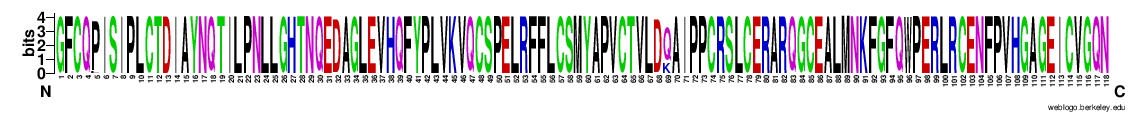
\includegraphics[width=0.8\linewidth]{Figures/CRD_sequence_logo.png} 
    \caption{Cysteine rich domain consesus logo. Generated by \href{https://weblogo.berkeley.edu/logo.cgi}{WebLogo} }
    \label{fig:CRD-logo}
\end{figure}

\begin{figure}[H]
    % \centering
    
\includegraphics[width=0.8\linewidth]{Figures/hydrophobic_region_logo-2.png} 
    \caption{Hydrophobic domains consesus logo. Generated by \href{http://skylign.org/}{Skylign}}
    \label{fig:hydroDomains-logo}
\end{figure}

\begin{figure}[H]
    % \centering
    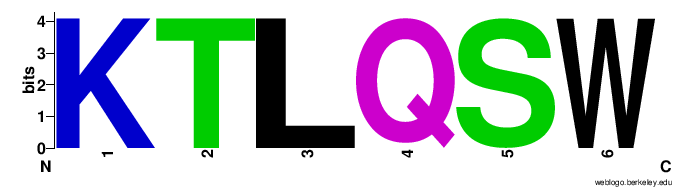
\includegraphics[width=0.8\linewidth]{Figures/KTXXXW.png} 
    \caption{KTXXXW motif consesus logo. Generated by \href{https://weblogo.berkeley.edu/logo.cgi}{WebLogo}}
    \label{fig:KTXXXW motif-logo}
\end{figure}

\end{document}
